\section{Theoretical Analysis}
\label{sec:theoretical}

\noindent \par In this section, the circuit shown in Figure~\ref{fig:V(t)} is analysed theoretically, considering the values shown in table \ref{tab1}.

\subsection{First point}
\label{ssec:1T}
\noindent \par In the first point, the goal is to perform node analysis for $t<0$, to determine all node voltages.
\par In order to do this, we did KCL in each node, considering that all currents were diverging from it, which lead us to the following matrix equation

\begin{equation}
\label{eq:teo1}
	\begin{bmatrix}
	1 & 0 & 0 & 0 & 0 & 0 & 0 & 0 \\ -G1 & G1+G2+G3 & -G2 & 0 & -G3 & 0 & 0 & 0 \\ 0 & -G2-Kb & G2 & 0 & Kb & 0 & 0 & 0 \\ 0 & 0 & 0 & 1 & 0 & 0 & 0 & 0 \\ 0 & 0 & 0 & Kd \cdot G6 & -1 & 0 & -Kd 		\cdot G6 & 1 \\ 0 & Kb & 0 & 0 & -Kb-G5 & G5 & 0 & 0 \\ 0 & 0 & 0 & -G6 & 0 & 0 & G6+G7 & -G7 \\ 0 & -G3 & 0 & -G4-G6 & G3+G4+G5 & -G5 & G6 & 0 \\
	\end{bmatrix}
	\begin{bmatrix}
	V1 \\ V2 \\ V3 \\ V4 \\ V5 \\ V6 \\ V7 \\ V8
	\end{bmatrix}
	=
	\begin{bmatrix}
	Vs \\ 0 \\ 0 \\ 0 \\ 0 \\ 0 \\ 0 \\ 0
	\end{bmatrix}
\end{equation}

\par Solving equation \ref{eq:teo1}, we get the following result

\begin{table}[h!]
\centering
\begin{tabularx}{0.6\textwidth} {
  | >{\raggedright\arraybackslash}X
  | >{\raggedleft\arraybackslash}X | }
 \hline
 V1 & 5.223200e+00 V \\ \hline
V2 & 4.960945e+00 V \\ \hline
V3 & 4.406214e+00 V \\ \hline
V4 & 0.000000e+00 V \\ \hline
V5 & 4.998463e+00 V \\ \hline
V6 & 5.852787e+00 V \\ \hline
V7 & -2.069080e+00 V \\ \hline
V8 & -3.074760e+00 V \\ \hline

\end{tabularx}
\end{table}

\par Knowing all node voltages, we can determine Ib, then use Ohm's law in resistors R1 and R6, and finally we can use mesh analysis to determine all branch currents.

\begin{figure}[h!] \centering
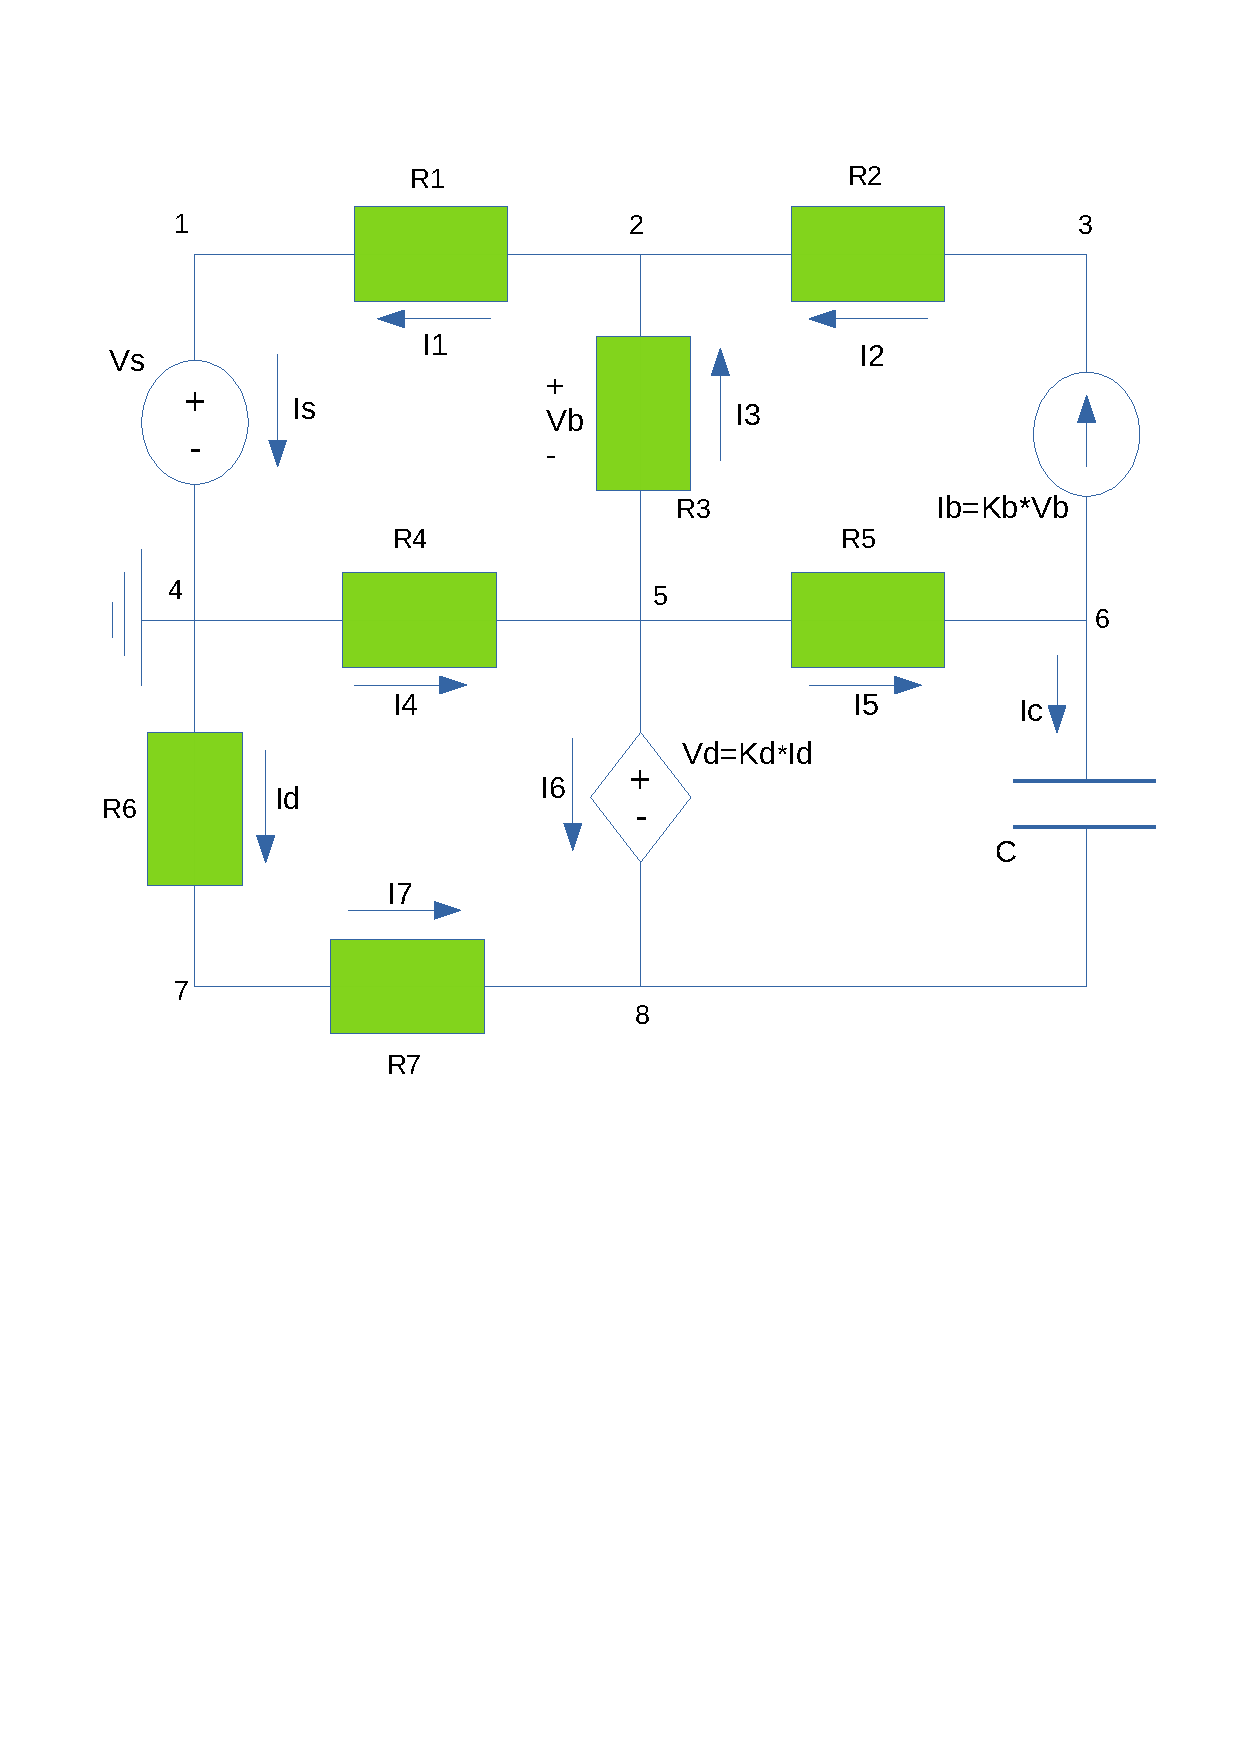
\includegraphics[width=0.6\linewidth]{Esquema1_currents_teo.pdf}
\caption{Current directions considered to determine all branch currents}
\label{fig:Esquema1_currents_teo}
\end{figure}

\par Considering the current directions shown in figure \ref{fig:Esquema1_currents_teo}, we get the following result

\begin{table}[h!]
\centering
\begin{tabularx}{0.6\textwidth} {
  | >{\raggedright\arraybackslash}X
  | >{\raggedleft\arraybackslash}X | }
 \hline
 I1 & -2.604926e-04 A \\ \hline
I2 & -2.728588e-04 A \\ \hline
I3 & 1.236617e-05 A \\ \hline
I4 & -1.248639e-03 A \\ \hline
I5 & -2.728588e-04 A \\ \hline
I6 & 9.881466e-04 A \\ \hline
I7 & 9.881466e-04 A \\ \hline
Is & -2.604926e-04 A \\ \hline
Ic & 0.000000e+00 A \\ \hline
Id & 9.881466e-04 A \\ \hline

\end{tabularx}
\end{table}


	


